% Section content template for individual Educative lessons
% This file contains the actual content for a specific section
% Generated from Educative API section content

% Section: Activity Diagram for  Facebook
% Section ID: 4550266590593024
% Section Slug: activity-diagram-for-facebook
% Generated: 2025-12-14T12:40:16.559133

Activity diagrams are a great way to visualize the flow of messages from one activity to another in the system. There can be different activity diagrams that we can create for Facebook. In this lesson, we will create activity diagrams for the following two activities:

\begin{itemize}
\item
\protect\phantomsection\label{Y8TrLubIbQArxxwZcV6KK}
Creating a new post.
\item
\protect\phantomsection\label{7q_TZoPKdRc6QP2shnORT}
\textbf{Activity challenge:} A user joins a group.
\end{itemize}

\subsection{Creating a new post}\label{cSJPCzl4S0TQDrKL8ZFax}
\\
The states and actions involved in this activity diagram are provided below.

\subsubsection{States}\label{ixgWMDgnjnUgud7gHOv-F}
\\
\textbf{Initial state:} The user selects the new post option.
\\
\textbf{Final state:}~The post is published.

\subsubsection{Actions}\label{N0OIOFlKEjsEVCCUO-ONB}
\\
The user selects the new post option, selects the privacy option, adds any attachments, and publishes the post.

\begin{figure}[htbp]
 \centering
 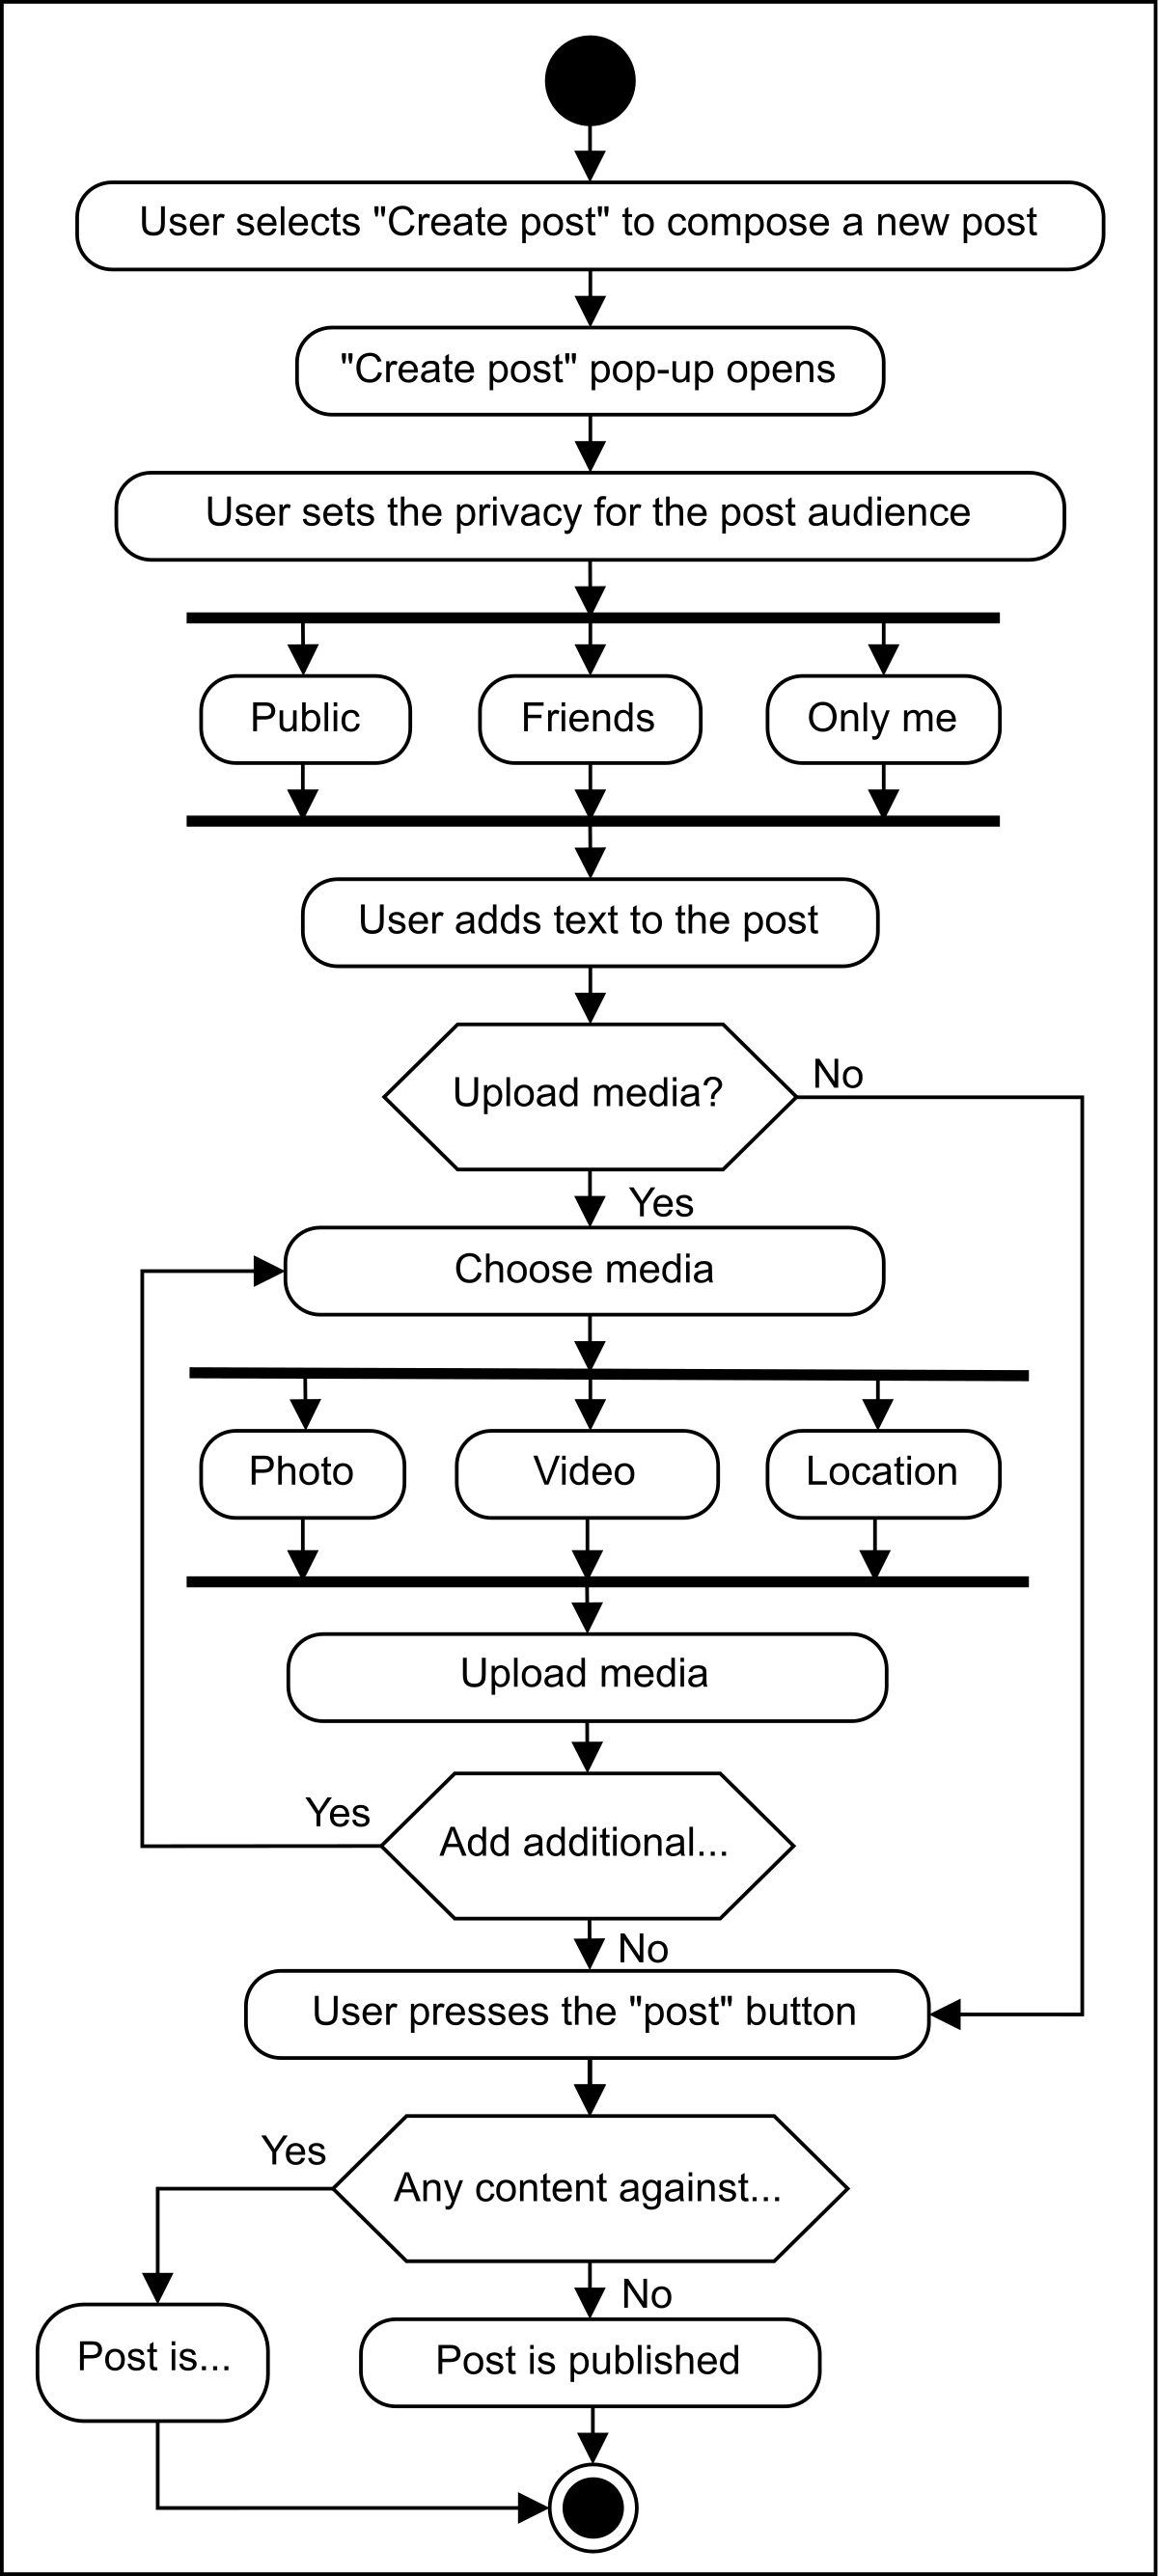
\includegraphics[width=0.5\textwidth]{Images/chapter_22/section_4550266590593024/4580658069635072.png}
 \caption{The activity diagram for a user creating a new post}
\end{figure}

\subsection{Activity challenge: A user joins a group}\label{6VHUkhcIzLoTXBpIRHVKK}
\\
You'll help us create an activity diagram of a user joining a group. A skeleton of the activity diagram is given below:

\begin{figure}[htbp]
 \centering
 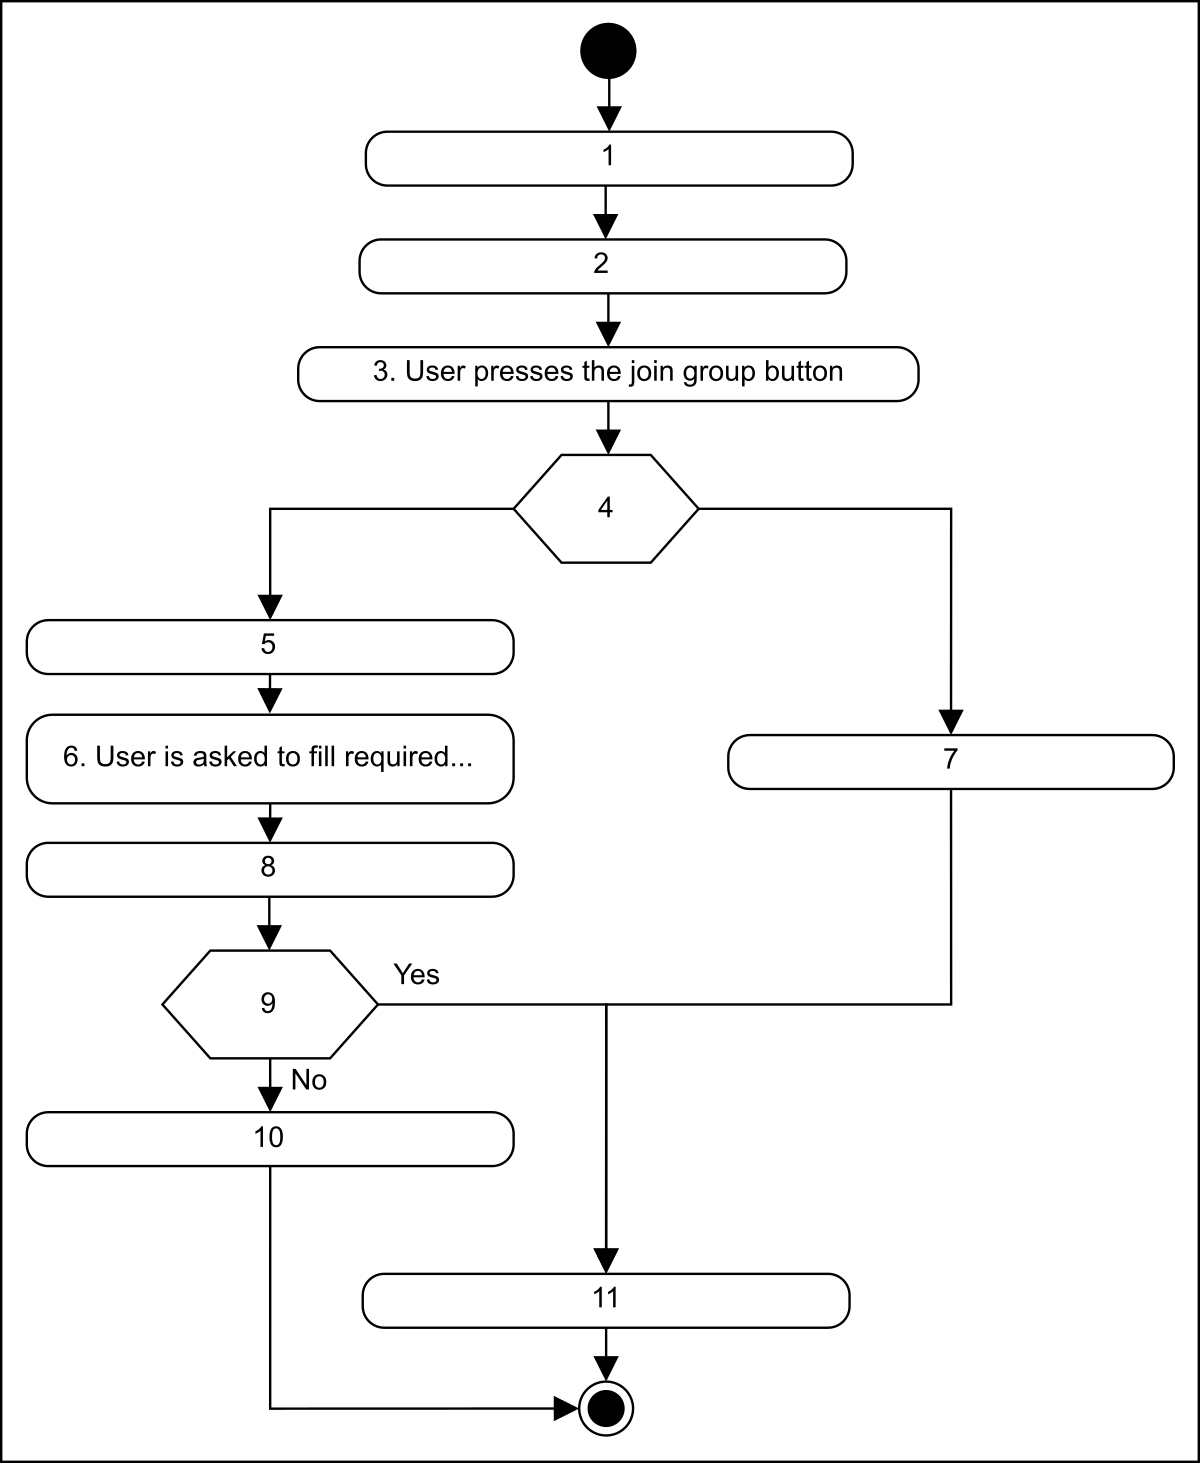
\includegraphics[width=0.5\textwidth]{Images/chapter_22/section_4550266590593024/5982314288119808.png}
 \caption{The activity diagram for a user joining the group}
\end{figure}

Notice that the actions in the diagram above are numbered from 1 to 11. The slots in the above diagram represent the activities, and the arrows represent the flow from one activity to the other.
\\
Can you rearrange the slots below into the correct order in which they should appear in the activity diagram above?
\begin{quote}
\textbf{Note:} If you're stuck, click the ``Show Solution'' button.
\end{quote}

\textit{Component type 'Permutation' not yet supported.}

Alternatively, you can click the ``Show complete diagram'' button below to see the complete activity diagram.

We've looked at some of Facebook's activity diagrams. In the next lesson, we will present the code for our designed classes in some of the most popular languages.

% End of section content